\documentclass[11pt,a4paper]{article}

\usepackage{iftex}
\ifTUTeX
  \usepackage{fontspec}
  \setmainfont{texgyretermes}[Extension=.otf, UprightFont=*-regular, BoldFont=*-bold,
    ItalicFont=*-italic, BoldItalicFont=*-bolditalic]
\else
  \usepackage[T1]{fontenc}
  \usepackage[utf8]{inputenc}
\fi
\usepackage[margin=2.4cm]{geometry}
\usepackage{amsmath,amssymb}
\usepackage{booktabs}
\usepackage{tabularx}
\usepackage{array}
\usepackage{graphicx}
\usepackage{caption}
\usepackage{enumitem}
\usepackage[hidelinks]{hyperref}
\usepackage{xurl}
\emergencystretch=2em

\captionsetup{font=small,labelfont=bf}
\setlist{nosep,leftmargin=*}
\newcolumntype{L}{>{\raggedright\arraybackslash}X}
\newcommand{\code}[1]{\texttt{#1}}

\title{Generating sub-resolution detail for GRACE/GRACE-FO water storage with a conditional
  diffusion model: octave transfer and model-trained detail}
\author{H. Oğuz Bolat}
\date{Progress report, draft for discussion\\[2pt] 18 November 2026}

\begin{document}
\maketitle

\begin{abstract}
\noindent
We investigate whether a conditional diffusion model can add realistic spatial detail to
GRACE and GRACE-FO terrestrial water storage (TWS) fields below the resolution of the
observations, and attach an honest uncertainty to that detail. Two approaches are examined. The
first, octave transfer, trains the model to add one octave of spherical-harmonic detail at
coarse scales, where GRACE resolves both input and target, and applies it unchanged one octave
finer. At its training scale the model outperforms all reference methods (continuous ranked
probability score, CRPS, 20.5\,mm against 45.9\,mm for a spectral Gaussian baseline), but one
octave finer it is worse than that baseline (52.5 against 48.7\,mm) and its ensembles are
markedly over-confident, whereas a model trained at the finer scale itself
reaches 24.8\,mm. The same behaviour is found on a hydrological-model twin free of GRACE noise
and filtering, so the failure reflects a change of the scale relation rather than a property
of the observations. In the second approach the network is trained on ten global hydrological
models from ISIMIP3a and applied to GRACE, with a consistency projection that keeps GRACE's
coarse coefficients exactly. At scales where GRACE can still be used as reference, this
network improves on the spectral baseline by 7--10\,mm CRPS and recovers a substantial part of
the observed detail (correlation 0.64--0.73), but its ensemble spread is about two thirds of
its error. Calibrating the spread is the next step, followed by tests at the target scales.
\end{abstract}

\section{Introduction}

GRACE and GRACE-FO resolve monthly mass change to a spatial scale of a few hundred
kilometres; below that, noise and the filtering needed to suppress it remove the signal. Many
hydrological applications, for example basin-scale groundwater assessment, require finer
detail. A generative model conditioned on the observed field can supply such detail as an
ensemble of plausible realisations that are consistent with the observation at the scales it
resolves, with the ensemble spread expressing the uncertainty of what is added.

The difficulty is that there are no observations at the scales to be generated, so a model
cannot be trained against them directly. This report examines two ways of obtaining training
examples. The first exploits scale relations within GRACE itself: if the relation between a
field and its next finer octave were similar across scales, a model trained where GRACE
resolves both could be applied where it does not (Part~I, Section~\ref{sec:part1}). The second
takes the fine-scale examples from global hydrological models, which resolve these scales, and
uses GRACE only as the conditioning input (Part~II, Section~\ref{sec:part2}). Data and methods
common to both parts are described in Sections~\ref{sec:data} and~\ref{sec:methods}.

The analysis is restricted to single months (no temporal modelling) and to GRACE-derived inputs.
All scores reported here are computed on validation years; the test years and the test region
(Section~\ref{sec:masks}) have not been used.

\section{Data}\label{sec:data}

\subsection{GRACE/GRACE-FO}
We use the ITSG-Grace2018 (April 2002 to June 2017, 162 months) and ITSG-Grace\_operational
(June 2018 to September 2026, 98 months) unconstrained monthly solutions to degree 120, 260
months in total. $C_{20}$, and $C_{30}$ where available, are replaced by the satellite laser
ranging values of GSFC TN-14, each calendar month taking the TN-14 entry whose time span
overlaps it most. Glacial isostatic adjustment is removed with the expectation model of Caron
et~al.\ (2018). Anomalies are taken relative to the 2004--2009 mean and converted to equivalent
water height (EWH) with PREM load Love numbers; degrees 0 and 1 are excluded. Two versions are
kept, unfiltered and DDK5-filtered, both truncated at degree 64. After 300\,km Gaussian
smoothing, the linear trends behave as expected: the GIA correction reduces the trend over
Hudson Bay from $+31.2$ to $-0.6$\,mm\,yr$^{-1}$ and over Scandinavia from $+21.8$ to
$+0.1$\,mm\,yr$^{-1}$. The choice of products is provisional.

\subsection{Hydrological models}
Part~I uses WaterGAP v2.2e (GSWP3-W5E5 forcing, historical human water use) as a closed-loop
twin: monthly TWS from 1901 to 2019 at $0.5^\circ$, on land only, regridded to a
Driscoll--Healy grid and expanded to degree 128. Because the twin contains clean fine-scale
signal, it can be scored at scales that GRACE does not resolve. In Part~I it is never used to
train the models applied to GRACE.

Part~II uses ten models of the ISIMIP3a global water sector, all driven by the same forcing and
protocol (GSWP3-W5E5, \code{obsclim}, \code{histsoc}), monthly TWS at $0.5^\circ$ for
1901--2019: CWatM, H08, HydroPy, JULES-ES-VN6P3, JULES-W2, LPJmL5-7-10-fire, MIROC-INTEG-LAND,
ORCHIDEE-MICT, WaterGAP2-2e (identical to the twin) and WEB-DHM-SG. All models are processed in
the same way. Cells whose storage drifts by more than 1\,m between 1901--1910 and 2010--2019 are
set to zero anomaly; these are unbounded snow accumulation on glaciers and point-like urban
groundwater abstraction, and their number ranges from 68 (WEB-DHM-SG) to 5603 (JULES-ES) cells.
Anomalies are taken relative to 2004--2009 and degrees 0 and 1 are removed, as for GRACE.
JULES-ES has three to four times the variability of the other models; inspection shows genuine
variability rather than drift, and the model is retained. CWatM and MIROC show offsets early in
the twentieth century, which we attribute to spin-up; they lie in the training years and are
retained for now.

\subsection{Land-only GRACE}
The hydrological models carry no ocean signal and do not represent the ice sheets. For Part~II
we therefore also construct land-only GRACE fields: each month is synthesised at degree 128,
set to zero over the ocean, Greenland and Antarctica, and expanded again, after which degrees
0 and 1 are removed. These fields share the domain of the models.

\subsection{Masks and data splits}\label{sec:masks}
A test region over Türkiye (30--45$^\circ$N, 20--50$^\circ$E), enlarged by one half-wavelength
of the target degree, is excluded from training and from all scores reported here. Greenland
and Antarctica (south of 60$^\circ$S) are excluded from the training loss and the scores, and
scores are computed over land only. The data are split into contiguous blocks of months
(Table~\ref{tab:splits}), since neighbouring months are correlated.

\begin{table}[ht]
\centering\small
\caption{Data splits (number of months in brackets).}
\label{tab:splits}
\begin{tabular}{lccc}
  \toprule
  & training & validation & test (not used) \\
  \midrule
  GRACE & 2002-04 to 2019-12 (179) & 2020-01 to 2022-12 (36) & 2023-01 to 2026-09 (45) \\
  Hydrological models & 1901--1989 (1068) & 1990--2001 (144) & 2002--2019 (216) \\
  \bottomrule
\end{tabular}
\end{table}

\section{Methods}\label{sec:methods}

\subsection{Scale decomposition}
Spherical-harmonic degree $l$ corresponds to a half-wavelength of about
$20\,000\,\mathrm{km}/l$. A field $x$ is limited to degree $L$ with a cosine taper, which avoids
the ringing of a sharp truncation:
\begin{equation}
  w_L(l) =
  \begin{cases}
    1, & l \le 0.8L,\\[2pt]
    \tfrac12\bigl[1 + \cos\bigl(\pi\,\tfrac{l - 0.8L}{0.2L}\bigr)\bigr], & 0.8L < l < L,\\[2pt]
    0, & l \ge L.
  \end{cases}
\end{equation}
One resolution step doubles the degree. Its input is the field limited to $L/2$, its target
the field limited to $L$, and the detail to be generated is $d = w_L x - w_{L/2} x$. We
label the steps R1 to R5 (Table~\ref{tab:steps}). GRACE resolves R1--R3; R4 and R5 are
accessible only in the hydrological models.

\begin{table}[ht]
\centering\small
\caption{Resolution steps. Grid sizes are latitude $\times$ longitude.}
\label{tab:steps}
\begin{tabular}{lllll}
  \toprule
  step & degrees & finest half-wavelength & grid & available in \\
  \midrule
  R1 & 4 $\to$ 8    & $\sim$2500\,km & $32\times64$    & GRACE, models \\
  R2 & 8 $\to$ 16   & $\sim$1250\,km & $64\times128$   & GRACE, models \\
  R3 & 16 $\to$ 32  & $\sim$625\,km  & $128\times256$  & GRACE, models \\
  R4 & 32 $\to$ 64  & $\sim$310\,km  & $256\times512$  & models \\
  R5 & 64 $\to$ 128 & $\sim$160\,km  & $512\times1024$ & models \\
  \bottomrule
\end{tabular}
\end{table}

Each step is represented on an equiangular Driscoll--Healy grid of $4L \times 8L$ points, so
that a feature at the target degree covers the same number of pixels at every step and a single
fully convolutional network can be applied to all of them. Since amplitudes decrease with
degree, each map is divided by the area-weighted root mean square (RMS) of its input and the
prediction is rescaled afterwards. During training, each month is rotated by a uniformly random
rotation of the sphere, applied exactly in the spectral domain, before synthesis on the grid;
the masks are rotated with the field. This augments the limited number of GRACE months,
distributes grid distortion over all features and prevents the network from memorising
geography. Scores are computed on unrotated fields.

\subsection{Consistency projection}
A generated field limited back to the input degree should reproduce the input. For every degree
with $w_{L/2}(l) > 0$, the coefficients of a generated field are therefore replaced by
$x^{\mathrm{in}}_l / w_{L/2}(l)$, which equals the true target coefficients because
$w_L(l) = 1$ on that range. The operation is a linear projection that leaves the true target
unchanged; it is applied to every ensemble member of every method. The remaining discrepancy is
of order $10^{-15}$\,mm. In Part~II this projection guarantees that GRACE alone determines the
coarse part of every output.

\subsection{Diffusion model}
The network is a U-Net with two input channels (the noisy detail and the conditioning input)
and one output channel, base width 64, channel multipliers (1, 2, 2, 4), two residual blocks per
level, group normalisation, SiLU activations and a Fourier-feature noise embedding, without
attention (16.3 million parameters). Padding is periodic in longitude and, across the poles,
reflects with a $180^\circ$ shift, so that convolutions see the true neighbours on the sphere.

The diffusion model follows the EDM formulation of Karras and co-workers. The denoiser is
\begin{equation}
  D(x;\sigma) = c_\mathrm{skip}(\sigma)\,x + c_\mathrm{out}(\sigma)\,
    F\bigl(c_\mathrm{in}(\sigma)\,x,\ \mathrm{input},\ \tfrac14\ln\sigma\bigr),
\end{equation}
with $c_\mathrm{skip} = \sigma_d^2/(\sigma^2+\sigma_d^2)$,
$c_\mathrm{out} = \sigma\sigma_d/\sqrt{\sigma^2+\sigma_d^2}$ and
$c_\mathrm{in} = 1/\sqrt{\sigma^2+\sigma_d^2}$, where $F$ is the U-Net and $\sigma_d$ the RMS of
the normalised training detail. The loss is
$\lambda(\sigma)\,\omega\,\lVert D(d + \sigma n;\sigma) - d\rVert^2$ with
$\lambda(\sigma) = (\sigma^2+\sigma_d^2)/(\sigma\sigma_d)^2$, $n \sim \mathcal N(0, I)$ and
pixel weights $\omega$ equal to cell area times the loss mask. Samples are drawn with the
deterministic second-order Heun solver in 32 steps from $\sigma_\mathrm{max}$ to 0.002
($\rho = 7$); ensemble members differ only in their initial noise.

The noise level during training is drawn from a log-normal distribution. Three schedules
were used (Table~\ref{tab:schedules}). The EDM default, tuned for natural images,
rarely produces the high noise levels at which the sampler determines the large-scale shape of
the output; Section~\ref{sec:p1diag} shows that this matters here.

\begin{table}[ht]
\centering\small
\caption{Training noise schedules.}
\label{tab:schedules}
\begin{tabular}{llcc}
  \toprule
  schedule & distribution of $\ln\sigma$ & $\sigma_\mathrm{max}$ & batches with $\sigma > 10$ \\
  \midrule
  default & $\mathcal N(-1.2,\ 1.2^2)$ & 80 & $\approx 0.2\%$ \\
  widened & $\mathcal N(-0.4,\ 1.6^2)$ & 20 & $\approx 4.5\%$ \\
  log-uniform & uniform on $[\ln 0.002,\ \ln 20]$ & 20 & $\approx 7.5\%$ \\
  \bottomrule
\end{tabular}
\end{table}

All networks are trained with AdamW (learning rate $2\times10^{-4}$, 1000 warm-up steps,
batch size 32, gradient clipping at 1) and an exponential moving average of the weights (decay
0.999). Each batch contains samples from a single resolution step chosen at random among the
training steps. The checkpoint with the lowest validation loss, evaluated every 2000 steps, is
retained. Training runs of 40\,000--60\,000 steps took 2--4\,h on an NVIDIA RTX 5090 (32\,GB).

\subsection{Reference methods}
Four reference methods are used.
(i) Input only: the input field without added detail; this sets the floor.
(ii) Spectral baseline: a power law is fitted to the degree variances of the input and
extrapolated to the missing degrees, and random coefficients with this spectrum are added to
the input. It has approximately correct power but no learned spatial structure, and since it
adapts to each month's spectrum it is a fair competitor at every step.
(iii) Climatological spectral baseline: as (ii), with the mean spectrum of the training months.
(iv) Regression U-Net: the same U-Net trained with a weighted mean squared error to predict $d$
directly, i.e.\ a deterministic estimate of the conditional mean.

\subsection{Evaluation}
Scores are computed on validation months in the original frame, weighted by cell area over
land outside the test region and the ice sheets, in mm EWH, and averaged over months.
Ensembles have 32 members (16 at R5).
The principal score is the continuous ranked probability score (CRPS), estimated per pixel with
the fair ensemble estimator
$\frac1M\sum_i|X_i - y| - \frac{1}{2M(M-1)}\sum_{i,j}|X_i - X_j|$; it rewards both accuracy and
appropriate spread and reduces to the absolute error for a single prediction. We further report
the RMSE of the ensemble mean and the correlation of the ensemble-mean detail with the true
detail; the spread/error ratio, i.e.\ the ensemble standard deviation over the ensemble-mean
RMSE, multiplied by $\sqrt{(M+1)/M}$, which is 1 for a calibrated ensemble and below 1 for an
over-confident one; and the coverage of the central 50\% and 90\% ensemble intervals from the
randomised probability integral transform. Methods are compared through the per-month CRPS
difference, with a 95\% interval from a moving-block bootstrap over months (blocks of 6 months
for GRACE and 12 for the models).

A method is regarded as successful when it improves on the spectral baseline with a bootstrap
interval excluding zero and its spread/error ratio lies between 0.85 and 1.15.

\section{Part I: octave transfer}\label{sec:part1}

\subsection{Design}
Networks are trained on R1 and R2 of the GRACE DDK5 fields and evaluated on R2 (the training
scale) and, without retraining, on R3, one octave finer. Before the experiment we specified
that transfer would be accepted if the network, at R3, (a) improved on the spectral baseline,
(b) came within 10\% of the CRPS of a network trained on R3 itself, and (c) had a spread/error
ratio between 0.85 and 1.15 with coverage within 5 percentage points of nominal. The
R3-trained network is not a candidate method, since such training data do not exist at the
target scales; it measures how well R3 detail can be learned and hence the cost of transfer.
The same experiment is repeated on the WaterGAP twin, where transfer can be followed to R4 and
R5.

\subsection{Results on GRACE}\label{sec:p1diag}
The first network, trained with the default noise schedule, appeared to transfer in part
(Table~\ref{tab:p1}): at R3 it improved on the spectral baseline by 3.3\,mm (95\% interval
$[-3.7, -2.9]$), and by 3.1\,mm on unfiltered GRACE, but it remained far from the R3-trained
network (45.5 against 24.8\,mm) and was over-confident (spread/error 0.82, coverage 40\% and
82\%). At its training scale, however, it was clearly inferior to the regression U-Net (37.2
against 26.3\,mm; ensemble-mean correlation 0.53 against 0.91), although the mean of a
well-trained diffusion ensemble should approach the regression estimate.

\begin{table}[ht]
\centering\small
\caption{GRACE DDK5, validation months. CRPS in mm; corr.\ is the correlation of the
ensemble-mean detail with the true detail. The last column gives the paired CRPS difference to
the spectral baseline at R3 with its 95\% bootstrap interval.}
\label{tab:p1}
\begin{tabular}{lrrrrrc}
  \toprule
  & \multicolumn{2}{c}{R2 (training scale)} & \multicolumn{3}{c}{R3 (one octave finer)} & \\
  \cmidrule(lr){2-3}\cmidrule(lr){4-6}
  method & CRPS & corr. & CRPS & corr. & spread/err. & difference at R3 \\
  \midrule
  input only & 62.9 & $-0.12$ & 64.0 & 0.18 & --- & \\
  spectral baseline & 45.9 & $-0.08$ & 48.7 & 0.13 & 1.23 & \\
  climatological spectral & 47.5 & $-0.10$ & 47.6 & 0.16 & 0.71 & \\
  regression U-Net & 26.3 & 0.91 & 71.1 & 0.25 & --- & \\
  diffusion, default schedule & 37.2 & 0.53 & 45.5 & 0.28 & 0.82 & $-3.3\ [-3.7, -2.9]$ \\
  diffusion, widened schedule & 20.5 & 0.90 & 52.5 & 0.21 & 0.37 & $+3.8\ [+2.7, +4.6]$ \\
  diffusion, log-uniform schedule & 21.6 & 0.89 & 51.0 & 0.23 & 0.49 & $+2.3\ [+1.7, +2.8]$ \\
  \midrule
  R3-trained reference & --- & --- & 24.8 & 0.86 & 0.88 & \\
  \bottomrule
\end{tabular}
\end{table}

Increasing the number of sampling steps from 32 to 128 left the result unchanged, which ruled
out the sampler. To examine what the network had learned, we applied its denoiser to pure noise
of a high level $\sigma$ together with a validation input. At such noise levels the output is
the network's own estimate of the detail given the input alone and can be compared directly with
the regression U-Net. At $\sigma = 10$ this estimate correlated only 0.26 (R1) and 0.40 (R2)
with the true detail, against 0.89 and 0.92 for the regression U-Net; the R3-trained network,
with the same schedule but four to sixteen times more pixels per batch, reached 0.79. Under the
default schedule only about 0.2\% of training batches have $\sigma > 10$, so the network had
barely learned to use its input in the regime where the sampler fixes the large-scale structure
of the output. The validation loss, dominated by low-noise cases, did not reveal this.

Retraining with the widened and log-uniform schedules (60\,000 steps) corrected the problem at
the training scale. The denoiser correlation at $\sigma = 10$ rose to 0.84 (R1) and 0.91 (R2),
the ensemble mean matched the regression U-Net (Figure~\ref{fig:diag}), and at R2 the diffusion
model became the best method tested (20.5\,mm). One octave finer, however, both retrained
networks are worse than the spectral baseline, with intervals excluding zero, and strongly
over-confident: the widened-schedule network has a spread/error ratio of 0.37 and its 50\% and
90\% intervals contain 21\% and 50\% of the truth. Their ensemble-mean correlation at R3 is
about 0.2, against 0.86 for the R3-trained network. Unfiltered GRACE gives the same picture.
The earlier partial success was therefore a consequence of the first network being weak: its
output was close to generic noise, which is roughly what the spectral baseline produces.
Figure~\ref{fig:crps} summarises the pattern: the better a network performs at its training
scale, the larger its loss one octave finer.

\begin{figure}[ht]
  \centering
  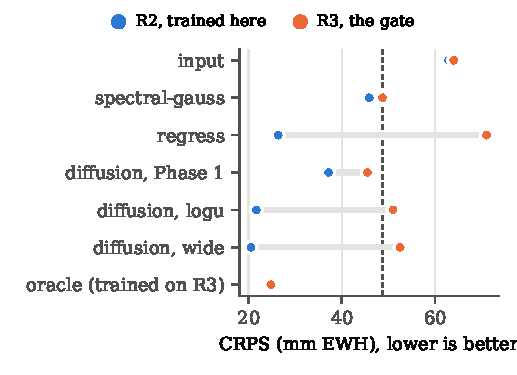
\includegraphics[width=0.55\linewidth]{figures/crps_r2_r3.pdf}
  \caption{GRACE DDK5: CRPS at the training scale R2 and one octave finer at R3. The dashed line
  marks the spectral baseline at R3.}
  \label{fig:crps}
\end{figure}

\begin{figure}[ht]
  \centering
  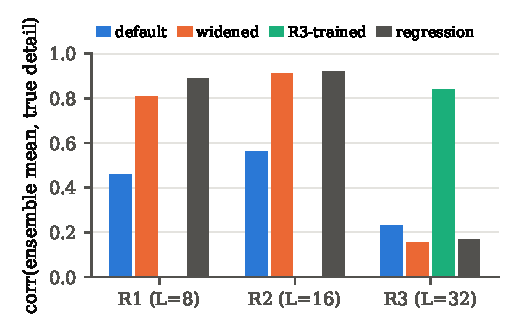
\includegraphics[width=0.55\linewidth]{figures/diagnosis_corr.pdf}
  \caption{Correlation of the ensemble-mean detail (for the regression U-Net, its prediction)
  with the true detail, GRACE DDK5 validation months. The widened schedule brings the diffusion
  model to the level of the regression U-Net at R1 and R2, but no network trained on R1 and R2
  carries this to R3, where the R3-trained network shows that the detail is learnable.}
  \label{fig:diag}
\end{figure}

\subsection{Results on the hydrological twin}
On the twin, the network trained with the default schedule improved on the spectral baseline
at every step from R2 to R5, but by a margin that decreased from 6.7\,mm at R2 to 0.8\,mm at
R4 and R5 (Table~\ref{tab:twin}, Figure~\ref{fig:twin}). As on GRACE, this network had the
weakness described above. Retrained with the widened schedule, it is far ahead at its training
scale (7.2 against 16.1\,mm, correlation 0.92) but ties with the spectral baseline at R3 and is
worse at R4, with spread/error ratios of 0.48 and 0.43. Its ensemble mean at R3 still carries
some structure (correlation 0.52 against 0.34 for the baseline, RMSE 25.9 against 28.3\,mm),
but the collapse of the spread cancels this gain in CRPS, and by R4 the structural advantage has
largely disappeared (0.36 against 0.31).

\begin{table}[ht]
\centering\small\setlength{\tabcolsep}{4pt}
\caption{WaterGAP twin, networks trained on R1 and R2, validation years. CRPS in mm;
differences to the spectral baseline with 95\% bootstrap intervals.}
\label{tab:twin}
\begin{tabular}{lrrrcrcc}
  \toprule
  & & & \multicolumn{2}{c}{default schedule} & \multicolumn{3}{c}{widened schedule} \\
  \cmidrule(lr){4-5}\cmidrule(lr){6-8}
  step & input & spectral & CRPS & difference & CRPS & difference & spread/err. \\
  \midrule
  R2 (training) & 21.2 & 16.1 & 9.4 & $-6.7\ [-6.9, -6.5]$ & 7.2 & $-8.9\ [-9.1, -8.6]$ & 0.85 \\
  R3 & 19.2 & 14.4 & 13.0 & $-1.4\ [-1.5, -1.2]$ & 14.5 & $+0.1\ [-0.2, +0.3]$ & 0.48 \\
  R4 & 19.6 & 15.0 & 14.1 & $-0.8\ [-0.9, -0.8]$ & 15.5 & $+0.5\ [+0.4, +0.6]$ & 0.43 \\
  R5 & 20.1 & 15.5 & 14.7 & $-0.8\ [-0.8, -0.7]$ & --- & --- & --- \\
  \bottomrule
\end{tabular}
\end{table}

\begin{figure}[ht]
  \centering
  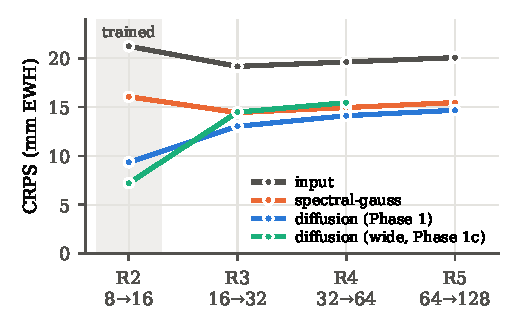
\includegraphics[width=0.55\linewidth]{figures/twin_rungs.pdf}
  \caption{WaterGAP twin: CRPS by resolution step for networks trained on R1 and R2 (shaded)
  and the reference methods.}
  \label{fig:twin}
\end{figure}

\subsection{Interpretation}
None of the networks trained on R1 and R2 satisfies the acceptance criteria at R3, and the
properly trained ones do not improve on the spectral baseline at all. Three observations explain
this outcome. First, the detail is learnable from data at its own scale: the R3-trained network
reaches 24.8\,mm against 48.7\,mm for the baseline on GRACE, and on the twin the network reaches
7.2 against 16.1\,mm at its training scale. A lack of information in the input is therefore not
the cause. Second, the learned relation does not carry over to the next octave, on GRACE or on
the twin. Since the twin contains neither GRACE noise nor the DDK filter, the failure is not an
artefact of the observations; the statistical relation between a TWS field and its next finer
octave evidently changes with scale, plausibly because the controlling structures (climate
zones, river basins, aquifers, topography) are not self-similar between 2500\,km and 300\,km, at
least as represented by WaterGAP. Third, the networks do not recognise that they are outside
their training distribution: one octave finer their ensembles are about half as wide as their
errors, so even partial structural skill is lost in CRPS.

We conclude that sub-resolution detail must be learned from examples at the scale concerned.
GRACE provides no such examples below about 500\,km, whereas global hydrological models do. A
methodological by-product is that the default EDM noise schedule was unsuitable for this
problem in a way the validation loss did not reveal; the denoiser diagnostic described above is
inexpensive and is now part of every evaluation.

\section{Part II: detail learned from hydrological models}\label{sec:part2}

\subsection{Approach}
The diffusion model is trained on hydrological-model TWS fields at the scales to be generated:
a model field is limited to GRACE's resolution and the network learns to restore the model's own
finer detail. At application, the network receives GRACE fields as input. The consistency
projection fixes all coarse coefficients to their GRACE values, so that GRACE determines the
large-scale field and the network contributes only the detail below its resolution, as an
ensemble. Several models are used jointly, so that the network learns properties common to the
models rather than the characteristics of one of them. GRACE thus serves as the conditioning
input, not as the training target.

The target is degree 128 (half-wavelength about 160\,km), reached from GRACE's degree 32 in two
single-octave stages, R4 and R5, each trained at its own scale on model data; no step relies on
transfer between scales.

The main risk is a mismatch between the coarse fields the network sees in training and those it
receives in application. Models and GRACE differ at large scales, notably in groundwater
depletion, long-term trends, glaciers and human water use, so GRACE inputs may lie outside the
distribution of model inputs. Using several models, masking the ice sheets and, if required,
perturbing the training inputs are intended to limit this mismatch. It must above all be
measured, which is possible only at scales where GRACE itself provides a reference.

The approach is assessed in four stages. G0 trains and tests on held-out years of the same models
at R4 and R5 and gives an upper bound without mismatch. G1 trains on the models at R2 and R3,
applies the network to GRACE and scores it against GRACE's own detail; it is the only stage
scored against observations. G2 trains on all models but one and tests on the held-out model at
R4 and R5, as a substitute for an independent world at scales GRACE cannot check. G3 applies the
full cascade to GRACE in the Türkiye test region and compares it with independent local data. G1
and G2 use the success criterion of Section~\ref{sec:methods}.

\subsection{First test at observable scales (G1)}
Two networks were trained on R2 and R3 with the widened schedule ($\sigma_\mathrm{max} = 20$,
60\,000 steps, about 3.5\,h each). The model-trained network was trained on the ten ISIMIP3a
models, each training sample being drawn from a randomly chosen model. A GRACE-trained network
was trained on land-only GRACE DDK5 over the GRACE training years; since such data will not exist
at the target scales, it serves as an upper bound. Both networks were applied to land-only GRACE
(DDK5 and unfiltered) and scored against GRACE's own detail over the 36 validation months. The
model-trained network was also applied to the full GRACE fields, including ocean and ice.

\begin{table}[ht]
\centering\small\setlength{\tabcolsep}{4pt}
\caption{G1: land-only GRACE, validation months 2020--2022. CRPS in mm. The last column gives
the paired difference between the model-trained network and the spectral baseline with its
95\% bootstrap interval.}
\label{tab:g1}
\begin{tabular}{llrrrrrc}
  \toprule
  & & & & \multicolumn{2}{c}{model-trained} & GRACE-trained & \\
  \cmidrule(lr){5-6}
  input & step & input only & spectral & CRPS & spread/err. & CRPS & difference \\
  \midrule
  DDK5 & R2 & 45.8 & 33.8 & 24.0 & 0.66 & 13.7 & $-9.9\ [-11.5, -8.5]$ \\
  DDK5 & R3 & 50.7 & 38.1 & 30.3 & 0.64 & 21.8 & $-7.9\ [-8.6, -7.1]$ \\
  unfiltered & R2 & 46.5 & 34.3 & 24.9 & 0.67 & 15.4 & $-9.4\ [-11.0, -8.0]$ \\
  unfiltered & R3 & 54.3 & 40.6 & 33.5 & 0.64 & 26.1 & $-7.1\ [-7.8, -6.3]$ \\
  \bottomrule
\end{tabular}
\end{table}

The model-trained network improves on the spectral baseline at both steps and for both GRACE
versions, by 7--10\,mm with intervals well clear of zero (Table~\ref{tab:g1}). Its ensemble mean
reproduces a substantial part of the observed detail, with correlations of 0.73 at R2 and 0.64
at R3 against 0.17 and 0.29 for the baseline. Training on several models is beneficial: at R2 on
land-only DDK5, the WaterGAP-only network of Part~I scores 28.0\,mm, the ten-model network
24.0\,mm. On the full GRACE fields at R3, the model-trained network still improves on the
spectral baseline (41.0 against 48.7\,mm; difference $-7.7$, interval $[-8.9, -6.6]$), which in
Part~I only the R3-trained network achieved. At R2 the improvement on full fields is small
($-1.6$\,mm, interval $[-2.7, -0.8]$), as the detail there is dominated by ocean and ice-sheet
signal that the models do not contain.

Two shortcomings remain. The model-trained network is 8--10\,mm behind the GRACE-trained network,
a measure of the mismatch between models and observations; the gap is smaller than the gain over
the baseline but not negligible. More importantly, its spread is too narrow: the spread/error
ratio is 0.64--0.67 and the nominal 90\% interval contains 72--76\% of the truth. The
GRACE-trained network is also somewhat over-confident (0.67--0.81), so the deficit is partly a
property of the method and not of the mismatch alone. G1 is therefore met with respect to skill
but not with respect to calibration.

\section{Discussion}

The two parts of this study lead to a consistent picture. Fine-scale TWS detail can be predicted
from the coarse field to a useful degree, but only by a network that has seen examples at the
relevant scale. Within GRACE, such examples do not exist below the resolution of the
observations, and the scale relation learned at coarser scales does not substitute for them. The
hydrological models provide the missing examples, and the G1 results show that detail learned
from models carries over to real GRACE fields at scales where this can be verified: the
model-trained network recovers detail that a structure-free baseline cannot, and the
consistency projection ensures that the observed coarse field is preserved exactly.

The common weakness of all learned ensembles in this study is calibration. In Part~I the
spread collapsed outside the training scale; in Part~II it is too narrow even where the network
performs well, and for the GRACE-trained network as well as the model-trained one. Because the
purpose of a generative model here is to express the uncertainty of the added detail, this is
the primary issue to resolve before moving to the target scales. Options that do not require
retraining are a stochastic sampler and an inflation of the ensemble spread about its mean;
inflation is compatible with the consistency projection because all members share the input's
coarse coefficients. An inflation factor fitted on GRACE would not, however, be available at
the target scales, where it must be derived from the models themselves (stage G2), and the
transferability of such a factor from models to GRACE has to be demonstrated at R2 and R3.

Several limitations apply. G1 tests the approach one and two octaves above the target scales;
whether the model-to-GRACE mismatch grows or shrinks at finer scales cannot be measured against
GRACE and must be inferred from G2 and from independent data in G3. The models disagree with
GRACE over the ocean and the ice sheets by construction, so the product is defined over land
only. The study treats months independently, does not yet include a test for spurious stripe
patterns or a two-sample test of generated against real detail, and omits degree-1 terms.

\section{Conclusions and further work}

Octave transfer, in which a model trained at coarse scales is applied one octave finer, is not
a viable basis for generating detail below GRACE's resolution: on GRACE and on clean model data
alike the learned skill does not transfer and the uncertainty does not widen to reflect this.
Learning the detail from an ensemble of hydrological models and conditioning on GRACE through an
exact consistency projection is a promising alternative. At scales where GRACE can serve as
reference, it improves on a spectral baseline by 7--10\,mm CRPS, though with ensembles that are
too narrow.

Further work will proceed in the following order: calibration of the ensemble spread on the
existing networks (stochastic sampling and spread inflation, fitted on GRACE training years and,
separately, on held-out model years); the leave-one-model-out test (G2) at R4 and R5; and the
application to the Türkiye test region (G3). The following points require a decision:
\begin{enumerate}
  \item confirmation of the hydrological models and the forcing protocol (currently ISIMIP3a,
    GSWP3-W5E5);
  \item the target resolution: degree 128 ($\sim$160\,km), or degree 256 ($\sim$80\,km), which
    would require models at $0.25^\circ$ or finer;
  \item the GRACE product and filter used as input;
  \item independent data for the Türkiye region (well levels, basin water budgets, regional
    products) for G3.
\end{enumerate}

\appendix
\section{Reproducibility}
Code is available at \url{https://github.com/hogib/GRACE_diffusion}. Part~I:
\code{scripts/phase1.sh}, \code{scripts/phase1b\_noise.sh} (noise schedules) and
\code{scripts/phase1c\_twin.sh} (twin, widened schedule); the denoiser diagnostic is
\code{scripts/diagnose\_sampler.py}. Part~II: model data are retrieved with
\code{python -m grace\_diffusion.fetch data/raw isimip} and prepared with
\code{python -m grace\_diffusion.prep data/raw data/proc isimip grace\_land}; the G1 runs are in
\code{scripts/g1\_models.sh}. Per-month scores are in \code{runs/eval/*.csv} and the figures
are produced by \code{reports/phase1/make\_figures.py}. Spherical-harmonic operations use
\code{pyshtools} and DDK filtering \code{shxarray}; networks use PyTorch 2.15.

\end{document}
